\newpage
\section{Критерий вполне ограниченности в больших Лебеговых пространствах}

\begin{claim}
	Пусть $K \subset \R^m$ --- выпуклый компакт, $C(K)$ --- непрерывные на $K$ функции с супремальной нормой. Пусть $S \subset C(K)$ таково, что 
	\begin{enumerate}
		\item $\exists M > 0: \ \forall f \in S :  \|f\|_c \leq M$
		\item $\forall f \in S \Rightarrow f \in C^1(K)$ и $\exists L > 0: \forall f \in S \Rightarrow \|\nabla f \|_c \leq L$
	\end{enumerate}
	Тогда $S$ --- вполне ограниченно в $C(K)$
\end{claim}
\begin{proof}
	По условию $S$ --- ограниченно, значит в силу теоремы Арцела-Асколе \ref{th:arzela} останется проверить равностепенную непрерывность. Возьмем произвольные $x,y \in K, |x-y| < \delta$ и рассмотрим $f(x) - f(y)$. Поскольку $K$ --- выпуклое множество, то 
	$$
	z(t) = y + t(x-y) \in K, \quad \forall t \in [0,1]
	$$
	Тогда 
	$$
	f(x) - f(y) = f(z(1)) - f(z(0)) = \int_{0}^{1} \frac{d}{dt}f(z(t))dt = \int_{0}^{1}\left(\nabla f(z(t)), \frac{d}{dt}z(t)\right) = \int_{0}^1(\nabla f(z(t)), x - y)
	$$
	$$
	|f(x)-f(y)| \leq \int_{0}^1|\nabla f(z(t))| |x-y| dt \leq L|x-y| \leq L\delta \leq \eps
	$$
	Где $\delta = \frac{\eps}{L}$, значит $S$ --- вполне ограниченно в $C(K)$
\end{proof}
\begin{theorem}[Рисс, Колмогоров]
	Пусть $1 \geq p \geq +\infty$, $S \subset \L_p(\R^m)$. Тогда $S$ --- вполне ограниченно в $\L_p(\R^m)$ тогда и только тогда когда
	\begin{enumerate}
		\item $S$ --- ограниченно в $\L_p(\R^m)$, то есть $\exists M > 0: \forall f \in S \Rightarrow \|f\|_p \leq M$
		\item $\forall \eps > 0 \ \exists R = R(\eps) > 0$: 
		$$
		\forall f \in S: \left(\int\limits_{\R^m \setminus B_{R(\eps)}(0)} |f(t)|^pdt\right)^\frac{1}{p} \leq \eps
		$$
		\item $\forall \eps > 0 \ \exists \delta(\eps) > 0$:
		$$
		\forall f \in S : \forall |z| \leq \delta \left(\int\limits_{\R^m} |f(t + z) - f(t)|^p dt\right)^\frac{1}{p}  \leq \eps
		$$
	\end{enumerate}
\end{theorem}
\begin{remark}
	При доказательстве дальнейших утверждений я иногда буду заменять $\eps$ на $\eps^p$ и наоборот, не оговаривая этого. Например в условии теоремы можно не извлекать корень из интегралов. Так как $p$ --- фиксированное число, то это ни на что не влияет. Делаю я это так как за этим зачастую запарно следить.
\end{remark}
Для доказательство нам потребуется следующее утверждение.
\begin{claim}[Достаточное условие вполне ограниченности в $\L_p(\R^m)$]
	Если $S \subset \L_p(\R^m)$ таково, что выполняются условия 1,2 теоремы Рисса-Колмогорова, а вместо 3 выполнено:
	$$
	S \subset C^{1}(\R^m), \ \exists L > 0: \forall f \in S :  \|\nabla f \|_p \leq L
	$$
	Тогда для $S$ будет выполнено условие 3.
\end{claim}
\begin{proof}
	Распишем разность как интеграл по формуле Ньютона-Лейбница:
	$$
	\int\limits_{\R^m}|f(t + z) - f(t)|^pdx = \int\limits_{\R^m}\left|\int_{0}^1\frac{d}{dt} f(x + tz)dt \right|^pdx \leq \int\limits_{\R^m} \left(\int_{0}^1 |\nabla f(x + tz)||z|dt\right)^pdx
	$$
	Применим неравенство Гельдера и вынесем $|z|^p$ как независимое от $x$ и $t$:
	$$
	\int\limits_{\R^m} \left(\int_{0}^1 |\nabla f(x + tz)||z|dt\right)^pdx \leq  |z|^p\int\limits_{\R^m}dx \int_0^1|\nabla f(x+tz)|^pdt
	$$
	Теперь применим теорему Фубини и сделаем замену $y = x + tz$:
	$$
	|z|^p\int\limits_{\R^m}dx \int_0^1|\nabla f(x+tz)|^pdt  =  |z|^p \int_{0}^1dt \int\limits_{\R^m}dy |\nabla f(y)|^p = |z|^p\int_{0}^1 \|\nabla f\|_p dt  \leq |z|^pL^p \stackrel{z \rr 0}{\rrr} 0 
	$$
\end{proof}
\begin{proof}[Доказательство теоремы Рисса-Колмогорова]
	Докажем необходимость. Пусть $S \subset \L_p(\R^m)$ --- вполне ограниченно в $\L_p(\R^m)$. Ограниченность следует из вполне ограниченности.  Дожем остальные условия. $\forall \eps > 0$ существует $\eps$-сеть:
	$$
	\exists g_1, \dots, g_M \in S
	$$
	Тогда по свойству интегрируемых по лебегу функций:
	$$
	\forall k \in \overline{1, M} \ \exists R_k > 0: \ \int\limits_{\R^m \setminus B_{R_k}(0)} |g_k|^p \leq \eps
	$$
	Тогда рассмотрев максимум этих чисел получим условие 2 для элементов сети. $R = \max\limits_{k \in \overline{1, M}}(R_k)$. $\forall k \in \overline{1, M}$:
	$$
	\int\limits_{\R^m \setminus B_{R}(0)} |g_k|^p \leq \eps
	$$
	Отсюда получаем что это свойство выполнено равномерно для всех элементов множества:
	$$
	\forall f \in S \exists k \in \overline{1, M}: \|f - g_k\|_p \leq \eps
	$$
	Далее я обозначаю корень из интеграла как норму, потому что это и есть норма на соответствующем пространстве:
	$$
	\|f\|_{\R^m \setminus B_{R}(0)} \leq \|f - g_k\|_{\R^m \setminus B_{R}(0)}  + \|g_k\|_{\R^m \setminus B_{R}(0)}  \leq \eps + \eps^p
	$$
	Что и требовалось для свойства 2. Аналогично по свойству интеграла лебега условие 3 выполнено для каждого элемента сети. $\forall \eps > 0 \ \exists \delta_k > 0$:
	$$
	\forall |z| \leq \delta_k \Rightarrow \|g_k(t+z) - g_k(t)\|_{\L_p(\R^m)} \leq \eps
	$$
	Тогда берем минимум $\delta = \min\limits_{k \in \overline{1, M}}$ и получаем условие 3 выполнено равномерно по всем элементам сети. Тогда 
	$$
	\forall f \in S \exists k \in \overline{1, M}: \|f - g_k\|_p \leq \eps
	$$
	И
	$$
	\|f(t+z) - f(t)\|_{\L_p(\R^m)}\leq \|f(t+z) - g_k(t+z)\|_{\L_p(\R^m)} + \|g_k(t+z) - g_k(t)\| + \|g_k(t) - f(t)\| \leq 3\eps
	$$
	Что и требовалось. Таким образом необходимость доказана. Пусть теперь выполнены свойства:
	\begin{enumerate}
		\item $S$ --- ограниченно в $\L_p(\R^m)$, то есть $\exists M > 0: \forall f \in S \Rightarrow \|f\|_p \leq M$
		\item $\forall \eps > 0 \ \exists R = R(\eps) > 0$: 
		$$
		\forall f \in S: \int\limits_{\R^m \setminus B_{R(\eps)}(0)} |f(t)|^pdt \leq \eps
		$$
		\item $\forall \eps > 0 \ \exists \delta(\eps) > 0$:
		$$
		\forall f \in S : \forall |z| \leq \delta \int\limits_{\R^m} |f(t + z) - f(t)|^p dt  \leq \eps
		$$
	\end{enumerate}
	Зафиксируем $\eps >0$ и $R = R(\eps) +\delta(\eps)$, где $R$ и $\delta$ из свойств 2 и 3 соответственно. Тогда по свойству 2: 
	$$
	\forall f \in S: \ \int\limits_{\R^m \setminus B_{R(\eps)}(0)} |f(t)|^pdt \leq \eps^p
	$$
	Тогда рассмотрим замкнутый шар в $\R^m$ радиуса $R$:
	$$
	K_P = \{x \in \R^m \mid |x| \leq R\}
	$$
	В $\R^m$ это компакт. Рассмотрим $C(K_R)$. Предположим мы нашли такое множество $S_\eps \subset C(K_R)$ --- вполне ограниченное в $C(K_R)$  что
	$$
	\forall f \in S: \exists \varphi \in S_\eps: \ \int\limits_{|x| \leq K_R} |f - \varphi|^p dx \leq \eps^p
	$$
	Тогда так как $S_\eps$ --- вполне ограниченно найдется $\frac{\eps}{\sqrt[p]{\mu (K_R)}}$-сеть для $S_\eps$ в $C(K_R)$, тогда мы можем построить 
	$$
	f_k(x) = \begin{cases}
		\varphi_k(x), x \in K_R \\
		0, x \notin K_R
	\end{cases}
	$$
	И это будет конечная сеть для $S$ в $\L_p(\R^m)$. Действительно 
	$$
	\forall f \in S: \exists \varphi \in S_\eps : \int\limits_{K_R}|f-\varphi|^p \leq \eps^p
	$$
	А для $\varphi \in S_\eps$ найдется такой $\varphi_k$, что:
	$$
	\|\varphi - \varphi_k\|_{C(K_R)} \leq \frac{\eps}{\sqrt[p]{\mu(K_R)}}
	$$
	Значит
	$$
	\|f - f_k\|_p \leq \sqrt[p]{\int\limits_{\R^m \setminus B_{R}(0)} |f|^p dx} + \sqrt[p]{\int\limits_{B_{R}(0)}\underbrace{|f - \varphi_k|^p}_{\pm \varphi}dx} \leq 
	$$
	$$
	\eps + \eps + \sqrt[p]{\int\limits_{K_R} |\varphi - \varphi_k|^p dx} \leq 2\eps + \sqrt[p]{\frac{\eps^p}{\mu(K_R)}\mu(K_R)} = 3\eps
	$$
	Значит $f_1, \dots f_M$ --- конечная $3\eps$-сеть для $S$ в $\L_p(\R^m)$. Заметим, что $f_k$ не обязаны лежать в $S$, но в силу замечания к определению вполне ограниченности нам это и не нужно.
	Остается доказать что такое $S_\eps$ найдется. Воспользуемся третьим свойством.  
	Построим функцию: 
		$$
	w (x) = \begin{cases}
		\exp \left( - \frac{|x|^2}{\delta^2 - |x|^2}\right), |x| \leq \delta \\
		0, |x| > \delta
	\end{cases}
	$$	
	Выглядит сложно, но на самом деле это просто шляпка такого вида:
	\begin{center}
		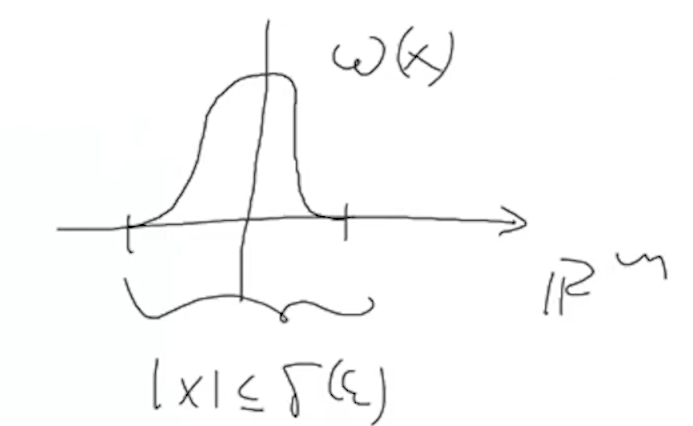
\includegraphics[width=0.5\textwidth]{pic/omega}
	\end{center}
	Она обладает хорошими свойствами: 
	\begin{itemize}
		\item $ w \in C^\infty(\R^m)$
		\item $\supp w = \{|x| \leq \delta\}$
		\item $\int\limits_{B_{\delta}(0)} w(x) dx = 1$
	\end{itemize}
	Теперь рассмотрим произвольную функцию $f \in S$ и свернем ее с функцией $w$:
	$$
	g_f(x) = \int\limits_{|y| \leq R} f(y)w(x-y)dy
	$$
	Тогда $g_f(x) \in C^\infty$ в частности:
	$$
	\nabla g_f(x) = \int\limits_{|y| \leq R} f(y) \nabla w (x-y) dy 
	$$ 
	Тогда рассмотрим:
	$$
	S_\eps = \{g_f \in C(K_R) \mid f \in S\}
	$$
	Функция $w$ ---  ограниченна, тогда
	$$
	\forall g \in S_\eps: |g(x)| \leq \alpha \int\limits_{B_{K_R}(0)} |f(x)|dx \leq \alpha \sqrt[p]{\int\limits_{B_{K_R}(0)}|f|^pdx} \sqrt[q]{\mu(K_R)} \leq \alpha M \sqrt[q]{\mu(K_R)}
	$$
	Значит $S_\eps$ ограниченно. Покажем равностепенную непрерывность. 
	$$
	|\nabla g| \leq \int\limits_{|y| \leq R} |f(y)| |\nabla w (x-y)| dy \leq \beta \int\limits_{|y| \leq R} |f(y)| dy \leq \beta M \sqrt[q]{\mu(K_R)} = \gamma
	$$
	Значит градиенты ограниченны, $\gamma$ --- общая для всех константа Липшица. Значит $S_\eps$ --- равностепенно непрерывно, и по теореме Арцела-Асколе получаем, что $S_\eps$ --- вполне ограниченно. Что и требовалось. Осталось показать, что 
	$$
	\forall f \in S: \exists \varphi \in S_\eps: \ \int\limits_{|x| \leq K_R} |f - \varphi|^p dx \leq \eps^p
	$$
	Заметим, что 
	$$
	g_f(x) = \int\limits_{|y| \leq R}f(y)w(x-y)dy = \int\limits_{\R^m}f_R(y)w(x-y)dy
	$$
	Где
	$$
	f_R = \begin{cases}
		f, \ x \in K_R, \\
		0, \ x \notin K_R
	\end{cases}
	$$
	Теперь сделаем замену $x - y = z$ и воспользуемся финитностью $w$:
	$$
	\int\limits_{\R^m}f_R(y)w(x-y)dy = \int\limits_{\R^m}f_R(x-z)w(z)dy = \int\limits_{|z| \leq \delta}f_R(x-z)w(z)dz 
	$$
	Тогда в силу того, что $\int\limits_{B_{\delta}(0)} w(x) dx = 1$ можно записать:
	$$
	\|f(t) - g_f(t)\|_{\L_p(K_R)} = \left\|\int\limits_{|z| \leq \delta} f(t)w(z)dz - \int\limits_{|z| \leq \delta} g_f(t) w(z) dz\right\|_{\L_p(|x|\leq R)}  = \left\| \int\limits_{|z| \leq \delta} (f(t) - f_R(t-z))w(z)dz\right\|_{\L_p(|x| \leq R)}
	$$
	Применяя неравенство Юнга-Минковского получаем:
	$$
	\|f(t) - g_f(t)\|_{\L_p(K_R)}  \leq \int\limits_{|z| \leq \delta} \|f(t) - f_R(t -z)\|_{\L_p(|x| \leq R)} 
	$$
	Под интегралом:
	$$
	\|\underbrace{f(t) - f_R(t -z)}_{\pm f(t-z)}\|_{\L_p(|x| \leq R)} \leq \|f(t)-f(t-z)\|_{\L_p(|x| \leq R)} + \|f(t-z) - f_R(t-z)\|_{\L_p(|x| \leq R}
	$$
	Рассмотрим каждое из слагаемых в первом применим условие 3, во втором условие 2: 
	$$
	\|f(t)-f(t-z)\|_{\L_p(|x| \leq R)} \leq \|f(t)-f(t-z)\|_p \leq \eps \ (|z| \leq \delta)
	$$
	$$
	 \|f(t-z) - f_R(t-z)\|_{\L_p(|x| \leq R} \leq \|f(t-z) - f_R(t-z)\|_p  = \|f - f_R\|_p = \sqrt[p]{\int\limits_{|y| > R} |f|^pdy} \leq \eps 
	$$
	Таким образом:
	$$
	\|f(t) - g_f(t)\|_{\L_p(K_R)} \leq 2\eps \int\limits_{|z|\leq \delta} w(z)dz  = 2\eps
	$$
	Таким образом, прорвавшись через тонны дерьма, мы получили необходимое $S_\eps$ и в силу рассуждений выше теорема доказана.
\end{proof}
\begin{next0}
	Пусть $E \subset \R^m$, $S \subset \L_p(E)$ тогда $S$ --- вполне ограниченно в $\L_p(E)$ тогда и только тогда когда:
	\begin{enumerate}
		\item $\exists M > 0, \forall f \in S \Rightarrow \|f\|_{\L_p(E)} \leq M$
		\item $\forall \eps > 0 \ \exists R > 0 \ \forall f \in S$:
		$$
		\int\limits_{|x| \leq R, x \in E} |f(x)|^p dx \leq \eps^p
		$$
		\item $\forall \eps > 0, \ \exists \delta :  \forall |z| \leq \delta, \ \forall f \in S$: 
		$$
		\| \Phi f (t + z) - \Phi f(t)\|_{\L_p(\R^m)} \leq \eps
		$$ 
		Где 
		$$
		\Phi : \L_p(E) \rr \L_p(\R^m), \quad \Phi f = \begin{cases}
			f(x), \ x\in E \\
			0, \ x \notin E
		\end{cases}
		$$
	\end{enumerate}
\end{next0}
\begin{proof}
	Ясно что:
	$$
	\|\Phi f\|_{\L_p(\R^m)} = \|f\|_{\L_p(E)}
	$$
	Тогда $\Phi$ --- изометрия. Применяя предыдущую теорему, получаем требуемое. 
\end{proof}

